
%----------------------------------------------------------------------------------------
%	CHAPTER 2
%----------------------------------------------------------------------------------------

\chapter{\textcolor{blue}{ \Bodycontrol~(Body control) em samba de gafieira }}

%%%%%%%%%%%%%%%%%%%%%%%%%%%%%%%%%%%%%%%%%%%%%%%%%%%%%%%%%%%%%%%%%%%%%%%%%%%%%%%%
%%%%%%%%%%%%%%%%%%%%%%%%%%%%%%%%%%%%%%%%%%%%%%%%%%%%%%%%%%%%%%%%%%%%%%%%%%%%%%%%
\section{ O corpo e suas relações}


Figura \ref{fig:bodycontroltotal}.

\begin{figure}[!h]
  \centering
    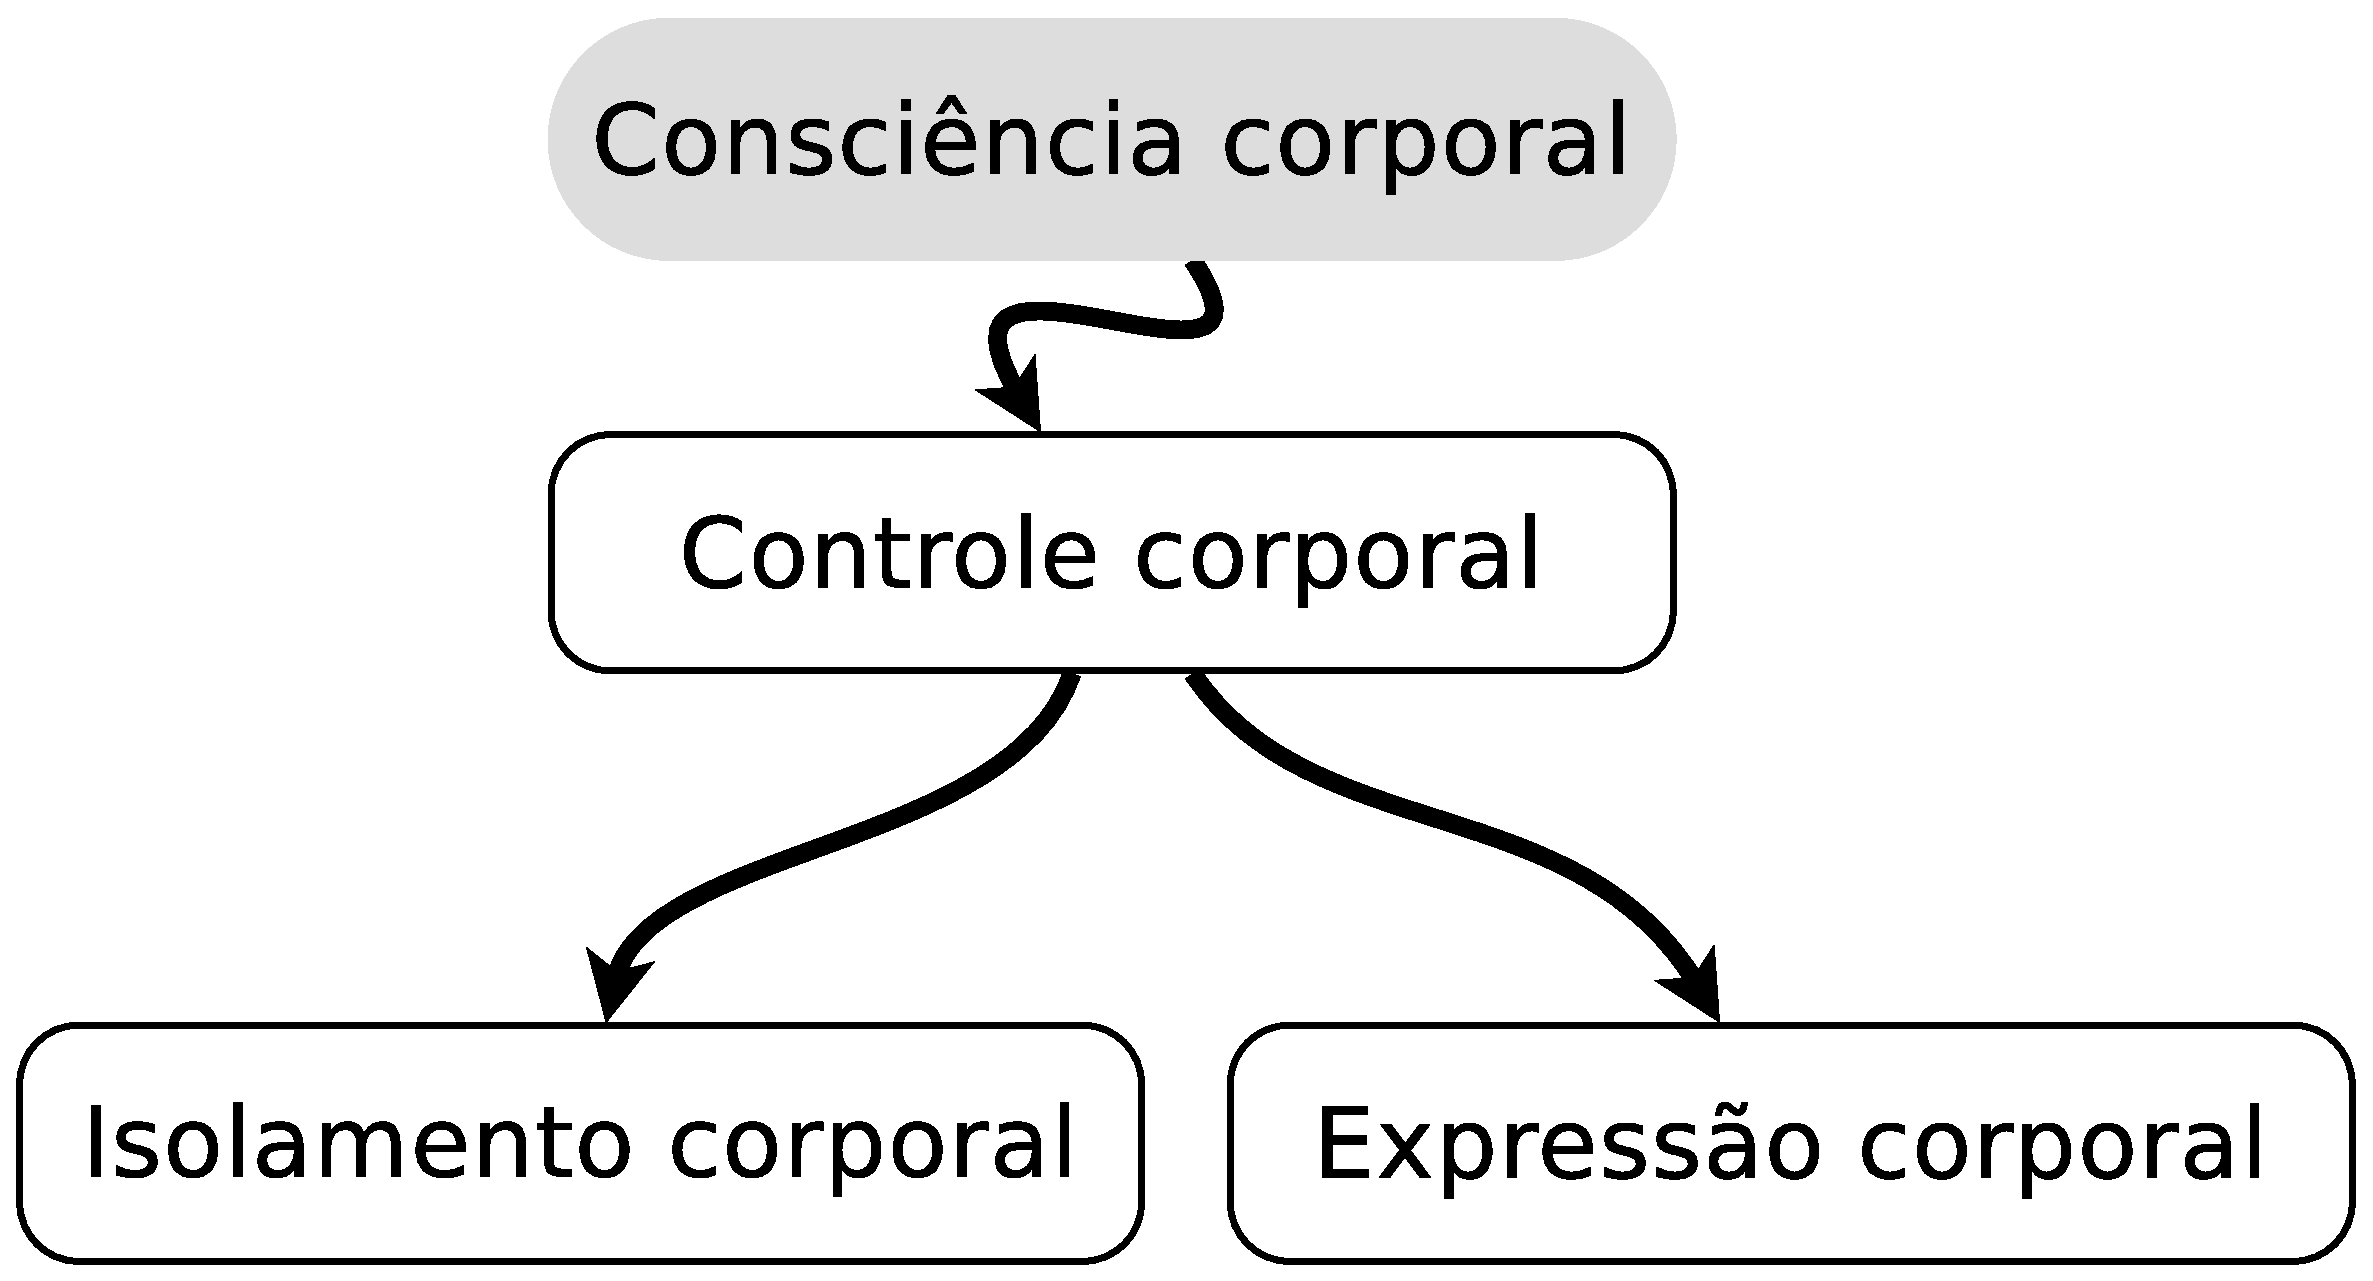
\includegraphics[width=0.5\textwidth]{chapters/cap-body-control/total.eps}
\caption{Relações do control corporal.}
\label{fig:bodycontroltotal}
\end{figure}


%%%%%%%%%%%%%%%%%%%%%%%%%%%%%%%%%%%%%%%%%%%%%%%%%%%%%%%%%%%%%%%%%%%%%%%%%%%%%%%%
\subsection{Que é consciencia corporal (Body awareness)}
\cite[pp. 11]{balcells2002expresion}
\cite{bueno2016psicomotricidade}
\cite[pp. 232]{gaiarsameio}
\cite[pp. 61]{aranha2002desenvolvimento}
\cite[pp. 75]{vallejo2001cuerpo}

%%%%%%%%%%%%%%%%%%%%%%%%%%%%%%%%%%%%%%%%%%%%%%%%%%%%%%%%%%%%%%%%%%%%%%%%%%%%%%%%
\subsection{Que é \Bodycontrol (Body control)}

\cite{bolio2006fantasia}
\cite[pp. 215]{moreno2008expresion}

%%%%%%%%%%%%%%%%%%%%%%%%%%%%%%%%%%%%%%%%%%%%%%%%%%%%%%%%%%%%%%%%%%%%%%%%%%%%%%%%
\subsection{Que é a expressão corporal}
\cite{balcells2002expresion}
\cite[pp. 215]{moreno2008expresion}

%%%%%%%%%%%%%%%%%%%%%%%%%%%%%%%%%%%%%%%%%%%%%%%%%%%%%%%%%%%%%%%%%%%%%%%%%%%%%%%%
\subsection{Que é a \bodyisolation}


%%%%%%%%%%%%%%%%%%%%%%%%%%%%%%%%%%%%%%%%%%%%%%%%%%%%%%%%%%%%%%%%%%%%%%%%%%%%%%%%
%%%%%%%%%%%%%%%%%%%%%%%%%%%%%%%%%%%%%%%%%%%%%%%%%%%%%%%%%%%%%%%%%%%%%%%%%%%%%%%%
\section{ Treino de ombros e quadril no plano frontal}

Figura \ref{fig:pessoalombroquadril1}.

\begin{figure}[!h]
  \centering
    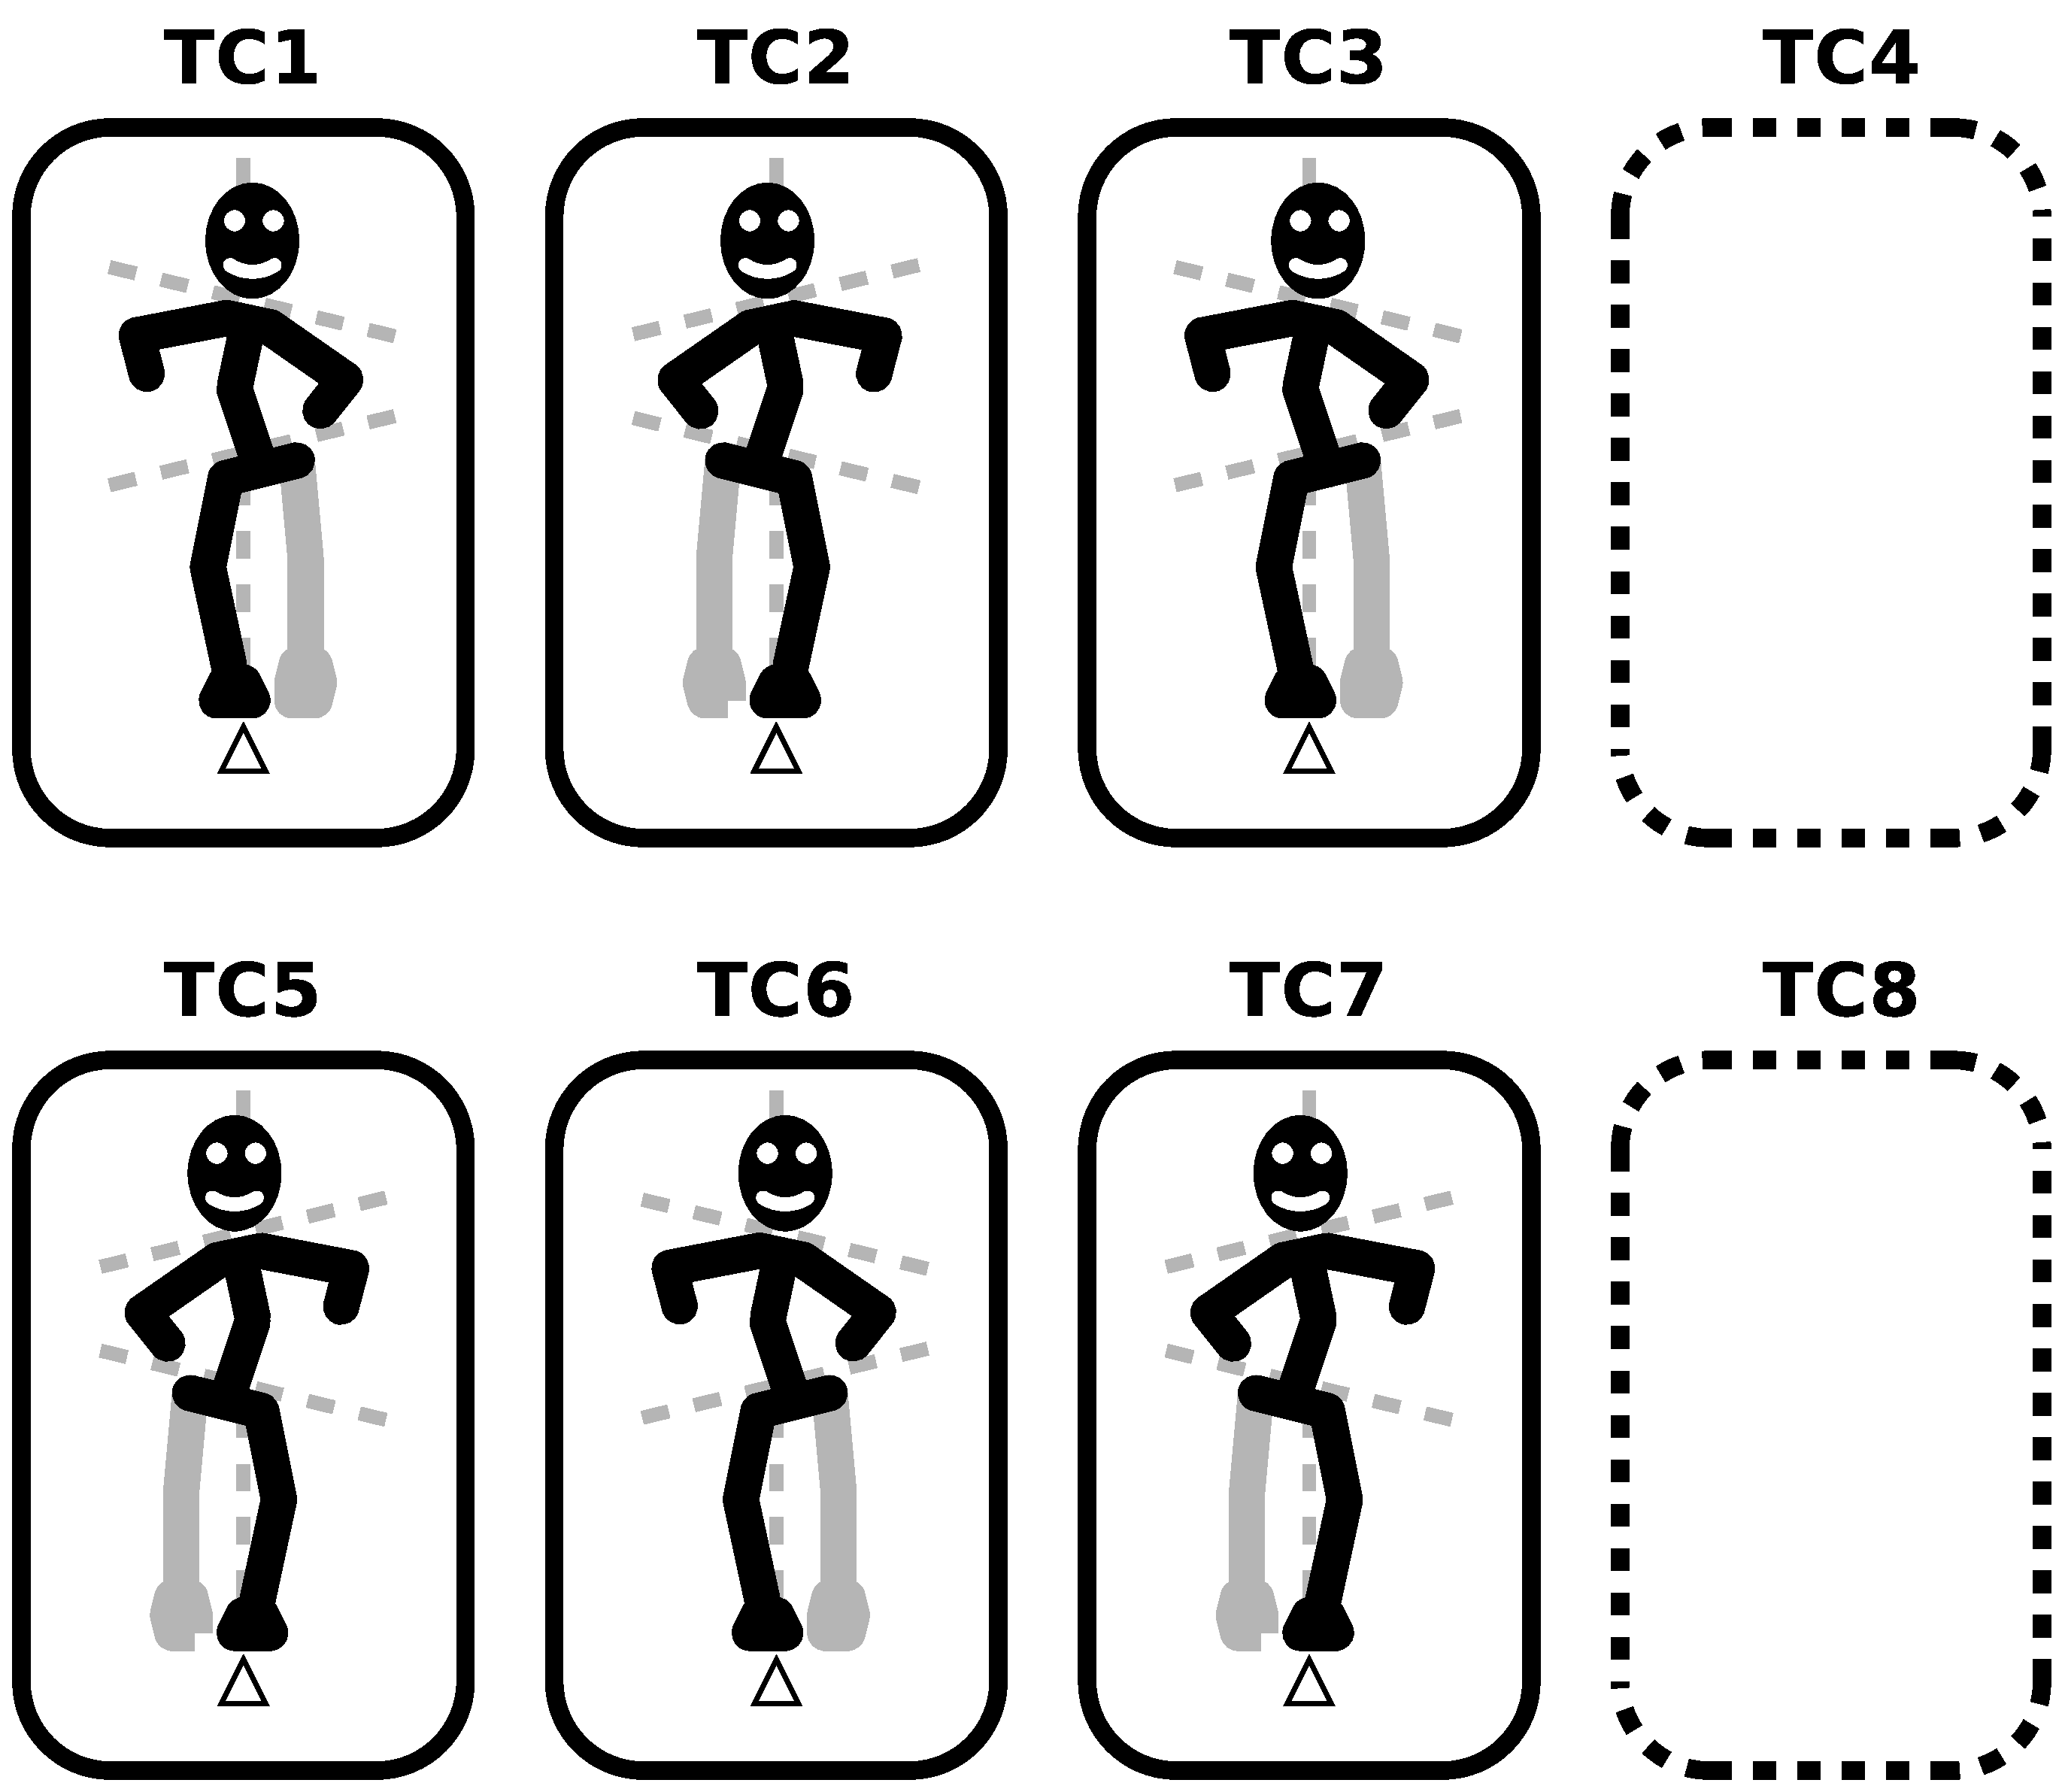
\includegraphics[width=\bodyboxsize]{chapters/cap-body-control/postura-ombro1.eps}
\caption{Diagrama de tempos coreográficos para o treino ombros e quadril, $T=2~TC$.}
\label{fig:pessoalombroquadril1}
\end{figure}

\section{\textcolor{red}{  Treino de ombros no plano frontal}}

\section{\textcolor{red}{  Treino do quadril no plano frontal}}




